% Elsevier CRC (Transportation Research Procedia) integrated manuscript
\documentclass[3p,times,procedia]{elsarticle}
\flushbottom

\usepackage{ecrc}
\usepackage{fancyhdr}
\pagestyle{fancy}
\fancyhf{}
\fancyfoot[R]{\thepage}
\renewcommand{\headrulewidth}{0pt}
\renewcommand{\footrulewidth}{0pt}

\volume{00}
\firstpage{1}
\journalname{Transportation Research Procedia}
\runauth{Zaman, Tomal, Chayan, Pandit, Cirillo}
\jid{trpro}

\usepackage{amssymb}
\usepackage{amsmath}
\usepackage{graphicx}
\usepackage{booktabs}
\usepackage{float}
\usepackage[figuresright]{rotating}
\usepackage{tikz}
\usetikzlibrary{positioning, arrows.meta, shapes.geometric}
\usepackage{caption}
\usepackage{siunitx}
\usepackage{array}
\usepackage{tabularx}
\captionsetup[table]{skip=8pt}
\graphicspath{{latex-images/}}
\usepackage[bookmarks=false,colorlinks,linkcolor=blue,citecolor=blue,urlcolor=blue]{hyperref}

\biboptions{numbers,sort&compress}

\begin{document}
\pagenumbering{arabic}
\begin{frontmatter}

\dochead{World Conference on Transport Research - Toulouse 6-10 July 2026}

\title{Weighted Mixed-Type VAE-Generated Trip Data for Agent-Based Road Assignment}

\author[a]{Raziq Zaman}
\ead{raziq@umd.edu}
\author[a]{Raas Sarker Tomal}
\ead{rtomal@umd.edu}
\author[a]{Md Mahmudul Huque Chayan}
\ead{mchayan@umd.edu}
\author[a]{Darshan Pandit}
\ead{dmpandit@umd.edu}
\author[a]{Cinzia Cirillo}
\ead{ccirillo@umd.edu}

\address[a]{Department of Civil and Environmental Engineering, University of Maryland}

\begin{abstract}
This study develops and evaluates a weighted, mixed-type Variational Autoencoder (VAE) for synthesizing person-trip records that can be converted into agent-based road-assignment inputs. The revised model treats continuous and nominal variables separately: numeric attributes are standardized and reconstructed with mean squared error, while categorical attributes are embedded, decoded through column-specific softmax heads, and trained with cross-entropy loss. This avoids imposing artificial ordinal distances on variables such as activity purpose, employment status, travel mode, and vehicle type. Household travel survey expansion weights are used during training and to set the population-scale number of synthetic trips; therefore, population and trip totals are control inputs rather than quantities inferred from the VAE. After preprocessing the Maryland Statewide Household Travel Survey and the Metropolitan Washington Council of Governments Regional Travel Survey, the modeling file contains \num{111808} long-format trip records and 79 modeled attributes. The trained VAE uses a 1800-dimensional standard-normal latent prior, four hidden layers with 2048, 1920, 1536, and 1024 units, categorical embeddings capped at 32 dimensions, and a beta-VAE loss with $\beta=0.01$. The deeper encoder and decoder are paired with a smaller training batch size of 512 and sampling batch size of 2048 to improve capacity while limiting GPU memory pressure. Sampling at the survey expansion scale produces \num{19103571} synthetic trip records, matching the weighted survey trip total of \num{19103571.28}. Distributional validation shows strong agreement for travel mode, vehicle occupancy, activity purpose, and reported travel time, while high-cardinality spatial fields remain more difficult. A car-only MATSim Stage 1 validation is revised to compare simulated link traversal speeds against direct observed speeds from the public VDOT 511 travel-time feed, rather than using volume-based proxies. The validation matches VDOT travel-time segments to OSM-derived MATSim links by route metadata and geometry, extracts simulated speeds from MATSim link-entry and link-exit events, and compares weighted-survey and VAE-synthetic demand using speed bias, MAE, RMSE, MAPE, correlation, and within-tolerance shares.
\end{abstract}

\begin{keyword}
Variational Autoencoder; Synthetic Trips; Mixed-Type Tabular Data; Household Travel Survey; MATSim; Traffic Speeds
\end{keyword}

\end{frontmatter}

\section*{Highlights}
\begin{itemize}
    \item A mixed-type VAE models numeric fields and nominal categories with separate loss terms.
    \item Survey weights set the population-scale trip count instead of asking the VAE to predict population totals.
    \item MATSim validation is framed as a car-only road-assignment and observed-speed test, not a full mode-choice model.
\end{itemize}

\newpage

\section{Introduction}
Understanding daily travel behavior is central to transportation planning, network investment, and policy evaluation. Activity-based and agent-based models represent travelers as individual decision makers whose trips and activities interact through time, space, and congestion. MATSim is one of the most widely used open-source platforms for such simulations because it can represent individual activity plans and simulate their interaction on a transport network \cite{horni2016matsim}.

The quality of an agent-based simulation depends heavily on the population and trip records used as inputs. Household travel surveys provide rich behavioral detail but are sparse relative to the population they represent. Survey weights can expand sample records to regional totals, but direct expansion reproduces survey idiosyncrasies, creates repeated records, and often provides limited support for local origin--destination, time-of-day, and activity combinations. Traditional population synthesis methods, including iterative proportional fitting and related reweighting methods, are useful for matching marginal control totals \cite{mueller2010synthetic}, but they are less suited to learning the joint relationships among trip purpose, location, departure time, household attributes, person attributes, and vehicle characteristics.

Deep generative models offer an alternative way to learn high-dimensional joint distributions from observed microdata. Variational Autoencoders (VAEs) are especially attractive because they provide a probabilistic latent representation and a direct sampling mechanism \cite{kingma_auto-encoding_2022}. However, tabular travel data contain a mixture of continuous fields and unordered categories. Treating all fields as integer values and optimizing a single mean squared error loss can impose false ordinal distances on nominal variables such as mode or activity purpose. In this paper, we therefore revise the model to use a mixed-type tabular VAE: numeric variables are reconstructed as standardized continuous values, whereas categorical variables are represented by embeddings and trained with cross-entropy loss.

The purpose of the methodology is not to infer the total population count. In practice, population and trip totals should come from external controls such as survey expansion weights, census products, observed traffic data, and planning forecasts. Our objective is narrower and more practical: generate a population-scale set of plausible trip records whose distributions and spatial-temporal patterns can be used as road-assignment demand in an agent-based simulator. The downstream MATSim exercise is correspondingly framed as a Stage 1 car-only network-loading validation against directly observed roadway speeds. It evaluates route loading and simulated link traversal speeds, not multimodal choice or long-run MATSim replanning equilibrium.

\section{Literature Review}\label{sec:lit-review}
Synthetic population and travel-demand generation has a long history in transport modeling. Travel surveys capture demographics, trip purposes, modes, times, and locations, while census and land-use sources provide more complete population controls. Classical approaches such as iterative proportional fitting, iterative proportional updating, rule-based expansion, and Markov-process methods remain common because they are interpretable and can match known marginals \cite{ramadan2019critical}. Their limitation is that they often require separate modules for population synthesis, trip generation, mode choice, and network assignment.

VAEs provide a probabilistic framework for learning joint distributions and sampling synthetic records \cite{kingma_auto-encoding_2022}. Early work on scalable population synthesis showed that VAEs can perform well in high-dimensional demographic spaces \cite{borysov_scalable_2019}. Subsequent studies compared VAEs with GAN-based alternatives \cite{garrido_prediction_2020}, explored rare-population coverage \cite{kim2022regularized}, and extended VAE architectures for household-individual synthesis \cite{sane2025joint}. Tabular models such as CTGAN and TVAE highlighted the value of column-specific treatment for mixed data \cite{xu_modeling_2019}. Recent work has also examined transferability, copula-augmented architectures, and systematic architecture sweeps \cite{jutras-dube_copula-based_2024,sane_comprehensive_2024}.

Trip-level synthesis remains less mature. Some studies use generative models for stop sequences, origin--destination patterns, or mobility traces \cite{chiesa2022gps,long2023dual,lestyan2022dp,badu-marfo_composite_2022}, but many approaches still separate demographic synthesis from trip generation. For agent-based transport simulation, this separation can reduce coherence between household attributes, person attributes, vehicle ownership, activity purpose, departure time, and origin--destination fields.

MATSim has been applied to many city and regional transport scenarios, including policy evaluation, emissions analysis, and synthetic-population validation \cite{w2016multi,horl2021synthetic,horl2025towards,felbermair2020generating,ziemke2019matsim}. In the present study, MATSim is used as an external validation environment: if VAE-synthesized trip records carry realistic spatial and temporal road demand, then their assigned link traversal speeds should preserve meaningful relationships with observed roadway speed data.

\section{Methods and Data}
\subsection{Survey Sources and Problem Definition}
The model combines two household travel surveys: the Maryland Statewide Household Travel Survey, conducted in 2018--2019 by the Baltimore Metropolitan Council \cite{baltimoremetropolitancouncilMarylandTravel}, and the Regional Travel Survey, conducted in 2017--2018 by the Metropolitan Washington Council of Governments \cite{mwcog}. The raw combined file contains \num{163290} long-format trip rows. After consolidation, column removal, required-field filtering, time conversion, and controlled blank filling, the modeling file contains \num{111808} trip rows and 80 columns, including the survey expansion weight \texttt{wthhfin}.

The large trip counts reported in this paper are weighted or generated population-scale counts, not raw survey sample sizes. The sum of the survey weights in the modeling file is \num{19103571.28}; the population-scale VAE sampler therefore generates \num{19103571} synthetic trip records. This design directly addresses the role of control totals: trip scale is supplied by the survey weights, while the VAE supplies the synthetic joint microstructure.

Transportation Analysis Zones (TAZs) are introduced here as the spatial unit used for home, work, school, origin, and destination locations. The implementation uses the Metropolitan Washington Transportation Planning Board TAZ layer. TAZ polygon centroids are fetched from the public MWCOG ArcGIS service and used as representative coordinates for MATSim plans. This centroid approximation avoids random point placement inside zones, but it also means that within-zone spatial dispersion is not represented in the current Stage 1 validation.

\subsection{Preprocessing Pipeline}
Figure~\ref{fig:pipeline} summarizes the implemented pipeline. The input surveys are first consolidated into a common flat schema. Person, household, trip, transit, vehicle, workplace, school, and delivery fields are retained where they are useful for modeling. Low-information identifiers and redundant variables are removed. Clock times are converted to minutes after midnight, survey dates are converted to days after January 1, 2017, and required TAZ fields are filtered to avoid invalid network locations. Remaining blanks are filled using controlled values: for example, no vehicle occupancy becomes zero, selected employment and smartphone fields receive survey-code defaults, and unresolved categorical blanks are represented as \texttt{N/A}.

\begin{figure}[H]
\centering
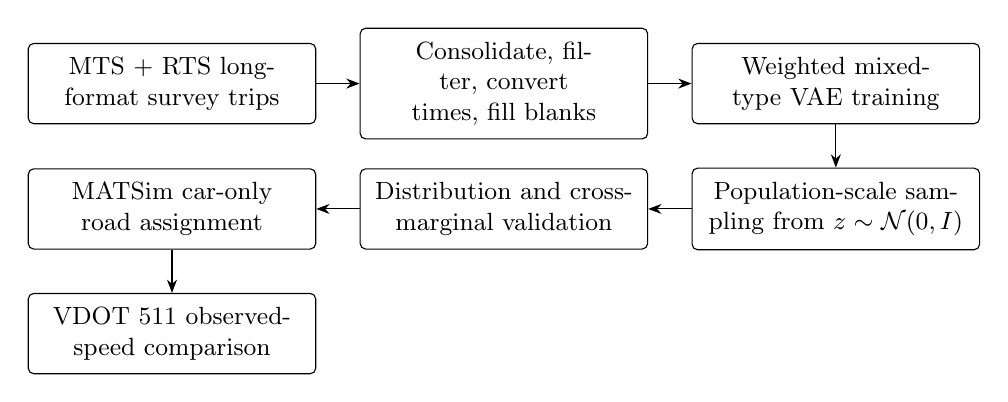
\begin{tikzpicture}[
    node distance=.55cm,
    every node/.style={draw, rounded corners=2pt, rectangle, font=\small, text width=3.3cm, align=center, inner sep=5pt},
    >=Stealth
]
\node (survey) {MTS + RTS long-format survey trips};
\node (prep) [right=of survey] {Consolidate, filter, convert times, fill blanks};
\node (vae) [right=of prep] {Weighted mixed-type VAE training};
\node (sample) [below=of vae] {Population-scale sampling from $z\sim\mathcal{N}(0,I)$};
\node (valid) [left=of sample] {Distribution and cross-marginal validation};
\node (matsim) [left=of valid] {MATSim car-only road assignment};
\node (counts) [below=of matsim] {VDOT 511 observed-speed comparison};
\draw[->] (survey) -- (prep);
\draw[->] (prep) -- (vae);
\draw[->] (vae) -- (sample);
\draw[->] (sample) -- (valid);
\draw[->] (valid) -- (matsim);
\draw[->] (matsim) -- (counts);
\end{tikzpicture}
\caption{\textbf{Implemented synthetic trip generation and validation pipeline.}}
\label{fig:pipeline}
\end{figure}

\subsection{Feature Representation}
The final model excludes the weight column from the decoder target and models 79 trip, household, person, vehicle, workplace, school, delivery, and transit-access attributes. The representation is mixed-type rather than all-integer. Twenty-four variables are modeled as numeric, standardized using their empirical mean and standard deviation. Fifty-five variables are modeled as categorical, including high-cardinality TAZ, vehicle make/model, activity-purpose, and travel-mode variables. Two numeric columns with remaining missingness, \texttt{year} and \texttt{td\_shop\_time}, receive explicit missingness indicators in the categorical part of the model.

\begin{table}[H]
\centering
\caption{Modeled feature groups in the long-format trip VAE.}
\label{tab:features}
\footnotesize
\begin{tabularx}{\linewidth}{p{3.0cm}X}
\toprule
\textbf{Group} & \textbf{Examples} \\
\midrule
Trip and activity & Origin and destination activity, departure time, reported travel time, travel mode, household and non-household travelers, vehicle occupancy, toll/HOV/parking fields. \\
Spatial fields & Origin TAZ, destination TAZ, home TAZ, workplace TAZ, school TAZ. \\
Vehicle fields & Body type, make, model, fuel type, model year, toll transponder. \\
Household fields & Household size, income, students, drivers, workers, disabilities, vehicles, bicycles, home type, home ownership. \\
Person fields & Age, gender, race and ethnicity, license, disability, employment, smartphone, student, school and workplace attributes. \\
Delivery and telework & Package, food, and service delivery indicators; telecommuting days and time; shopping time. \\
\bottomrule
\end{tabularx}
\end{table}

\subsection{Weighted Mixed-Type VAE}
The VAE follows the general tabular-VAE idea of learning a compressed latent representation and decoding synthetic rows \cite{xu_modeling_2019}, but it uses separate output heads for numeric and categorical data. Each categorical column has an embedding layer in the encoder. If a categorical variable has cardinality $K_j$, its embedding dimension is
\[
e_j=\min(32,\max(2,\lceil\sqrt{K_j}\rceil)).
\]
The numeric vector and all categorical embeddings are concatenated and passed through fully connected encoder layers of sizes 2048, 1920, 1536, and 1024 with layer normalization, ReLU activations, and dropout of 0.05. The encoder outputs a latent mean vector $\mu$ and log-variance vector $\log\sigma^2$ in an 1800-dimensional latent space. The decoder mirrors this depth in reverse order and produces one numeric head plus one categorical softmax head per categorical column.

\begin{figure}[H]
\centering
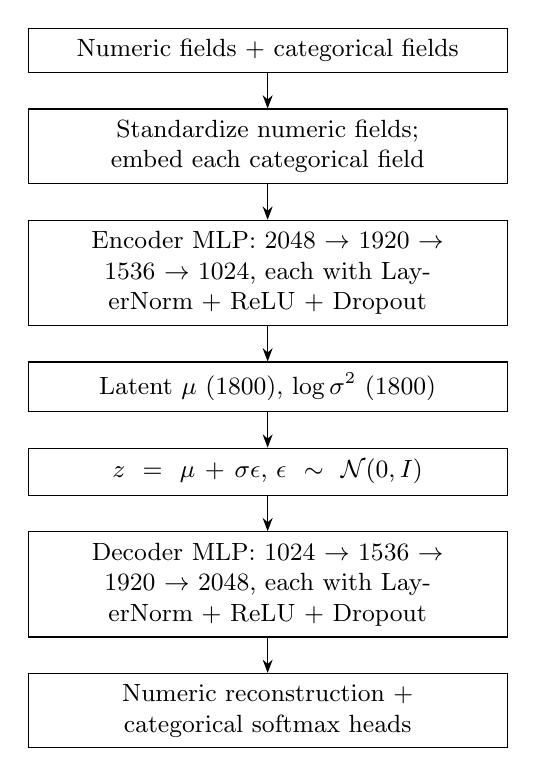
\begin{tikzpicture}[
    node distance=.45cm,
    every node/.style={draw, rectangle, font=\small, text width=5.8cm, align=center, inner sep=4pt},
    >=Stealth
]
\node (input) {Numeric fields + categorical fields};
\node (embed) [below=of input] {Standardize numeric fields; embed each categorical field};
\node (enc) [below=of embed] {Encoder MLP: 2048 $\rightarrow$ 1920 $\rightarrow$ 1536 $\rightarrow$ 1024, each with LayerNorm + ReLU + Dropout};
\node (latent) [below=of enc] {Latent $\mu$ (1800), $\log\sigma^2$ (1800)};
\node (sample) [below=of latent] {$z=\mu+\sigma\epsilon$, $\epsilon\sim\mathcal{N}(0,I)$};
\node (dec) [below=of sample] {Decoder MLP: 1024 $\rightarrow$ 1536 $\rightarrow$ 1920 $\rightarrow$ 2048, each with LayerNorm + ReLU + Dropout};
\node (out) [below=of dec] {Numeric reconstruction + categorical softmax heads};
\draw[->] (input) -- (embed);
\draw[->] (embed) -- (enc);
\draw[->] (enc) -- (latent);
\draw[->] (latent) -- (sample);
\draw[->] (sample) -- (dec);
\draw[->] (dec) -- (out);
\end{tikzpicture}
\caption{\textbf{Mixed-type VAE architecture used in the revised implementation.}}
\label{fig:architecture}
\end{figure}

Training uses a weighted random sampler with replacement, where each trip row $i$ is sampled with probability proportional to its expansion weight:
\[
p_i=\frac{w_i}{\sum_k w_k}.
\]
This allows the model to learn the weighted population distribution without treating the expansion weight as an output feature.

The loss combines numeric reconstruction, categorical reconstruction, and Kullback--Leibler regularization:
\[
\mathcal{L}=\mathcal{L}_{num}+\mathcal{L}_{cat}+\beta\mathcal{L}_{KL}, \qquad \beta=0.01.
\]
Here, $\mathcal{L}_{num}$ is mean squared error over standardized numeric fields, $\mathcal{L}_{cat}$ is the mean cross-entropy over categorical softmax heads, and
\[
\mathcal{L}_{KL}=-\frac{1}{2}\mathbb{E}\left[\sum_{\ell=1}^{1800}\left(1+\log\sigma^2_{\ell}-\mu_{\ell}^{2}-\sigma_{\ell}^{2}\right)\right].
\]
The standard-normal prior is used because it is the conventional VAE sampling prior and provides a smooth, directly sampleable latent space. The relatively high latent dimension and low $\beta$ were selected for this high-cardinality tabular setting to prioritize reconstruction of rare spatial and behavioral combinations while retaining stochastic sampling. They should be interpreted as the reported configuration rather than a universally optimal hyperparameter set.

The reported training configuration uses a maximum of 5040 epochs, batch size 512, sampling batch size 2048, initial learning rate $10^{-3}$, AdamW optimization, gradient clipping at norm 5, and random seed 2026. The trainer reduces the learning rate on loss plateaus down to a floor of $10^{-5}$ and applies early stopping after sustained non-improvement, so short within-epoch fluctuations are not interpreted as convergence failure. Figure~\ref{fig:training-loss} shows that the total loss, numeric loss, categorical loss, and KL term stabilize over training.

\begin{figure}[H]
\centering
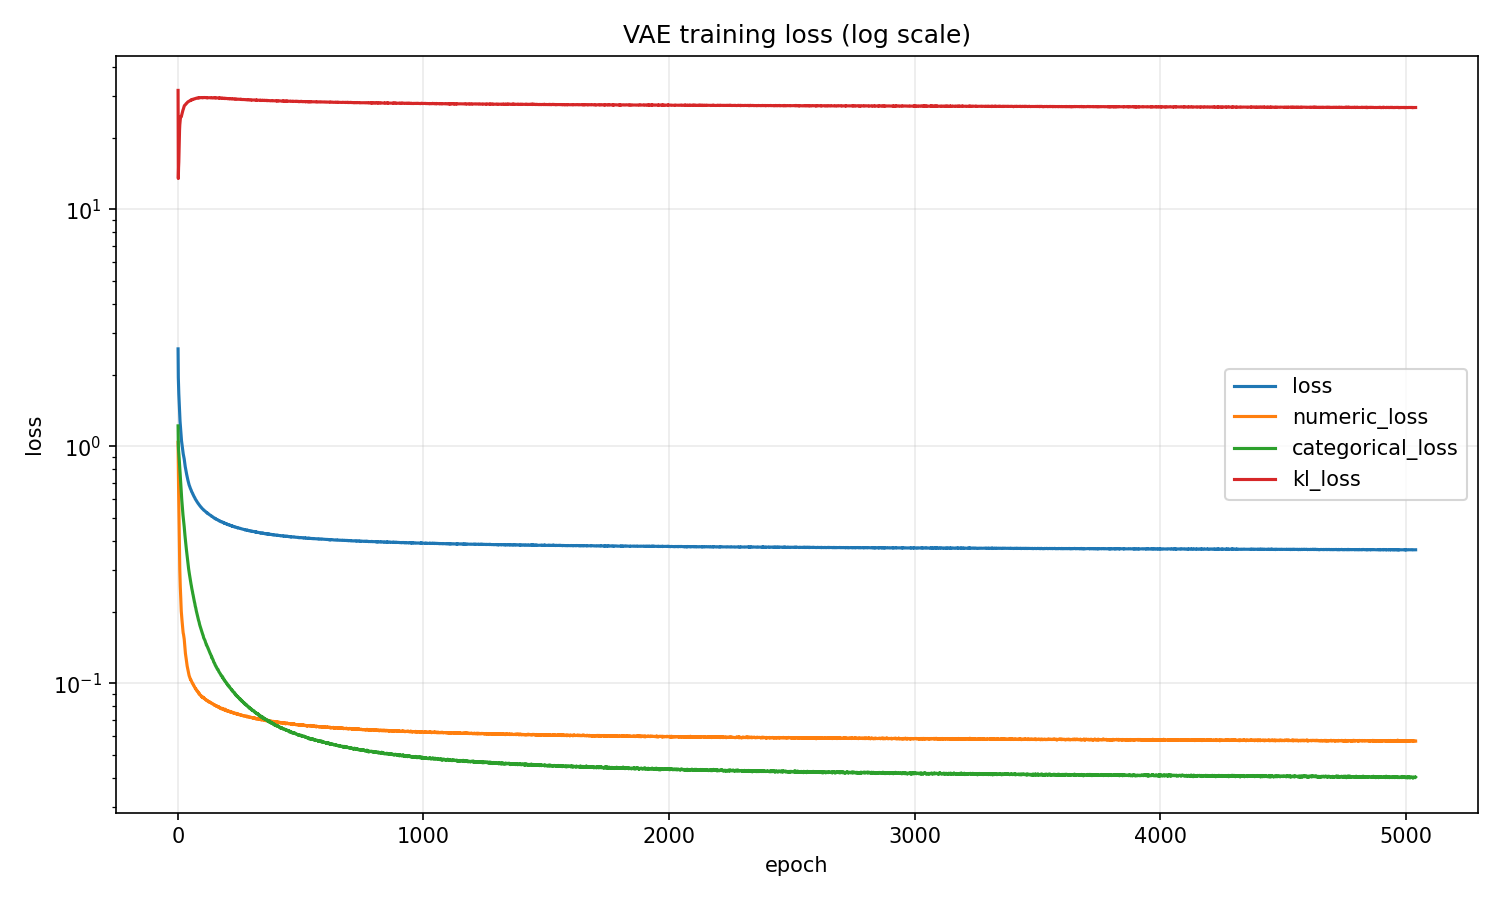
\includegraphics[width=.86\linewidth]{fig-training-loss-log.png}
\caption{\textbf{Training loss history for the weighted mixed-type VAE.}}
\label{fig:training-loss}
\end{figure}

\subsection{Sampling and Postprocessing}
After training, synthetic trips are generated by sampling $z\sim\mathcal{N}(0,I)$ and decoding each latent vector. Numeric outputs are de-standardized, clipped to the observed training range, and rounded where the underlying field is integer-valued. Categorical outputs are sampled from each column-specific softmax distribution, not rounded from arbitrary numeric codes. The population-scale sampler generates $\mathrm{round}(\sum_i w_i)=\num{19103571}$ trip rows.

\subsection{MATSim Road-Assignment Validation}
The MATSim validation is designed as a Stage 1 road-assignment test. It is not a full activity-based model calibration and does not include mode choice, transit assignment, departure-time replanning, or iterative coevolution. Only rows with positive vehicle occupancy are loaded onto the road network. A vehicle weight is computed as
\[
\text{vehicle weight}=\frac{\text{person-trip weight}}{\text{vehicle occupancy}}.
\]
For weighted survey rows, the person-trip weight is \texttt{wthhfin}. For population-scale synthetic rows, each generated trip has person-trip weight one. Fractional vehicle weights are expanded stochastically into ordinary unweighted MATSim car agents.

Each MATSim agent in this Stage 1 setup represents one vehicle trip: an origin activity at the origin TAZ centroid, a car leg, and a destination activity at the destination TAZ centroid. The network is built from OpenStreetMap PBF data \cite{openstreetmapOpenStreetMap}. The revised implementation can build a full state network or a smaller bounding-box network; the OSM-to-MATSim export now preserves link geometry, road class, length, free speed, capacity, name, reference route, and route-reference tags so that external speed segments can be matched to the simulated network.

Observed speeds are obtained directly from the public VDOT 511 travel-time feed rather than inferred from volume-based proxies. The implementation fetches \texttt{travel\_time\_response.json}, which contains current travel-time segment values including \texttt{avgSpeed}, and \texttt{travel\_time\_segments\_metadata.json}, which contains route descriptions and segment endpoint metadata. The source endpoints used by the code are \url{https://data.511-atis-ttrip-prod.iteriscloud.com/datasets/travelTime/travel_time_response.json} and \url{https://data.511-atis-ttrip-prod.iteriscloud.com/datasets/travelTime/travel_time_segments_metadata.json}. Because this public feed is a current operational snapshot rather than a licensed historical archive such as NPMRDS or RITIS, the fetched UTC timestamp and source URLs are written to every observed-speed row.

The speed-matching step first flattens the VDOT feed into segment-direction observations with route, description, start point, end point, observed speed, travel time, length, congestion, and imputation fields. Observed segments are then matched to OSM-derived MATSim links using route tokens from route names and reference tags when available, plus geometric segment-to-segment distance. The default maximum match distance is \SI{500}{m}. Direction is assigned by comparing the observed segment vector with the OSM link vector, producing a directed MATSim link identifier.

After MATSim runs, simulated speeds are extracted from link-entry and link-exit events. For every completed traversal of a directed link, travel time is the difference between the \texttt{entered link} and \texttt{left link} event times, and speed is computed as link length divided by traversal time. For each scenario, link speeds are summarized as traversal-weighted mean speeds and compared with the matched VDOT observed speeds. The primary comparison is between the weighted-survey baseline and the VAE synthetic demand under the same road network, demand geography, and MATSim configuration.

Model performance is evaluated with distributional overlap for input demand and with speed-specific assignment metrics for the MATSim validation: mean bias in mph, MAE, RMSE, MAPE, Pearson correlation, and the share of matched segments within 5~mph and 10~mph of observed VDOT speed. Distributional overlap remains
\[
O(P,Q)=\sum_b \min(P_b,Q_b)=1-\mathrm{TVD}(P,Q),
\]
where $P_b$ and $Q_b$ are real and synthetic proportions in bin or category $b$.

\section{Results and Discussion}
\subsection{Population-Scale Synthetic Trip Validation}
The population-scale sampler produces \num{19103571} synthetic trip records, matching the weighted survey trip total of \num{19103571.28}. This eliminates the earlier concern that the VAE was being asked to predict population scale. The scale is fixed by survey expansion weights; the VAE is evaluated on how well it reproduces the joint structure of the weighted trip records.

Table~\ref{tab:overlap-selected} reports selected population-scale distributional overlaps. Travel mode, vehicle occupancy, origin and destination activity, and reported travel time are closely matched. Spatial fields are more difficult because TAZ variables have thousands of categories and sparse origin--destination support.

\begin{table}[H]
\centering
\caption{Selected population-scale distributional overlaps.}
\label{tab:overlap-selected}
\footnotesize
\begin{tabular}{lcc}
\toprule
\textbf{Column} & \textbf{Overlap} & \textbf{Total variation distance} \\
\midrule
Vehicle occupancy & 0.976 & 0.024 \\
Travel mode & 0.968 & 0.032 \\
Destination activity & 0.935 & 0.065 \\
Reported travel time & 0.932 & 0.068 \\
Origin activity & 0.927 & 0.073 \\
Household income & 0.874 & 0.126 \\
Departure time & 0.857 & 0.143 \\
Distance & 0.829 & 0.171 \\
Origin TAZ & 0.779 & 0.221 \\
Destination TAZ & 0.769 & 0.231 \\
Home TAZ & 0.764 & 0.236 \\
\bottomrule
\end{tabular}
\end{table}

Figure~\ref{fig:labeled-mode-activity} shows labeled examples for travel mode and origin activity. The synthetic data preserve the dominance of auto-driver and auto-passenger trips and the major activity-purpose structure. The largest visible activity difference is an overrepresentation of home-origin trips and an underrepresentation of shopping-origin trips, which is consistent with the column-wise total variation results.

\begin{figure}[H]
\centering
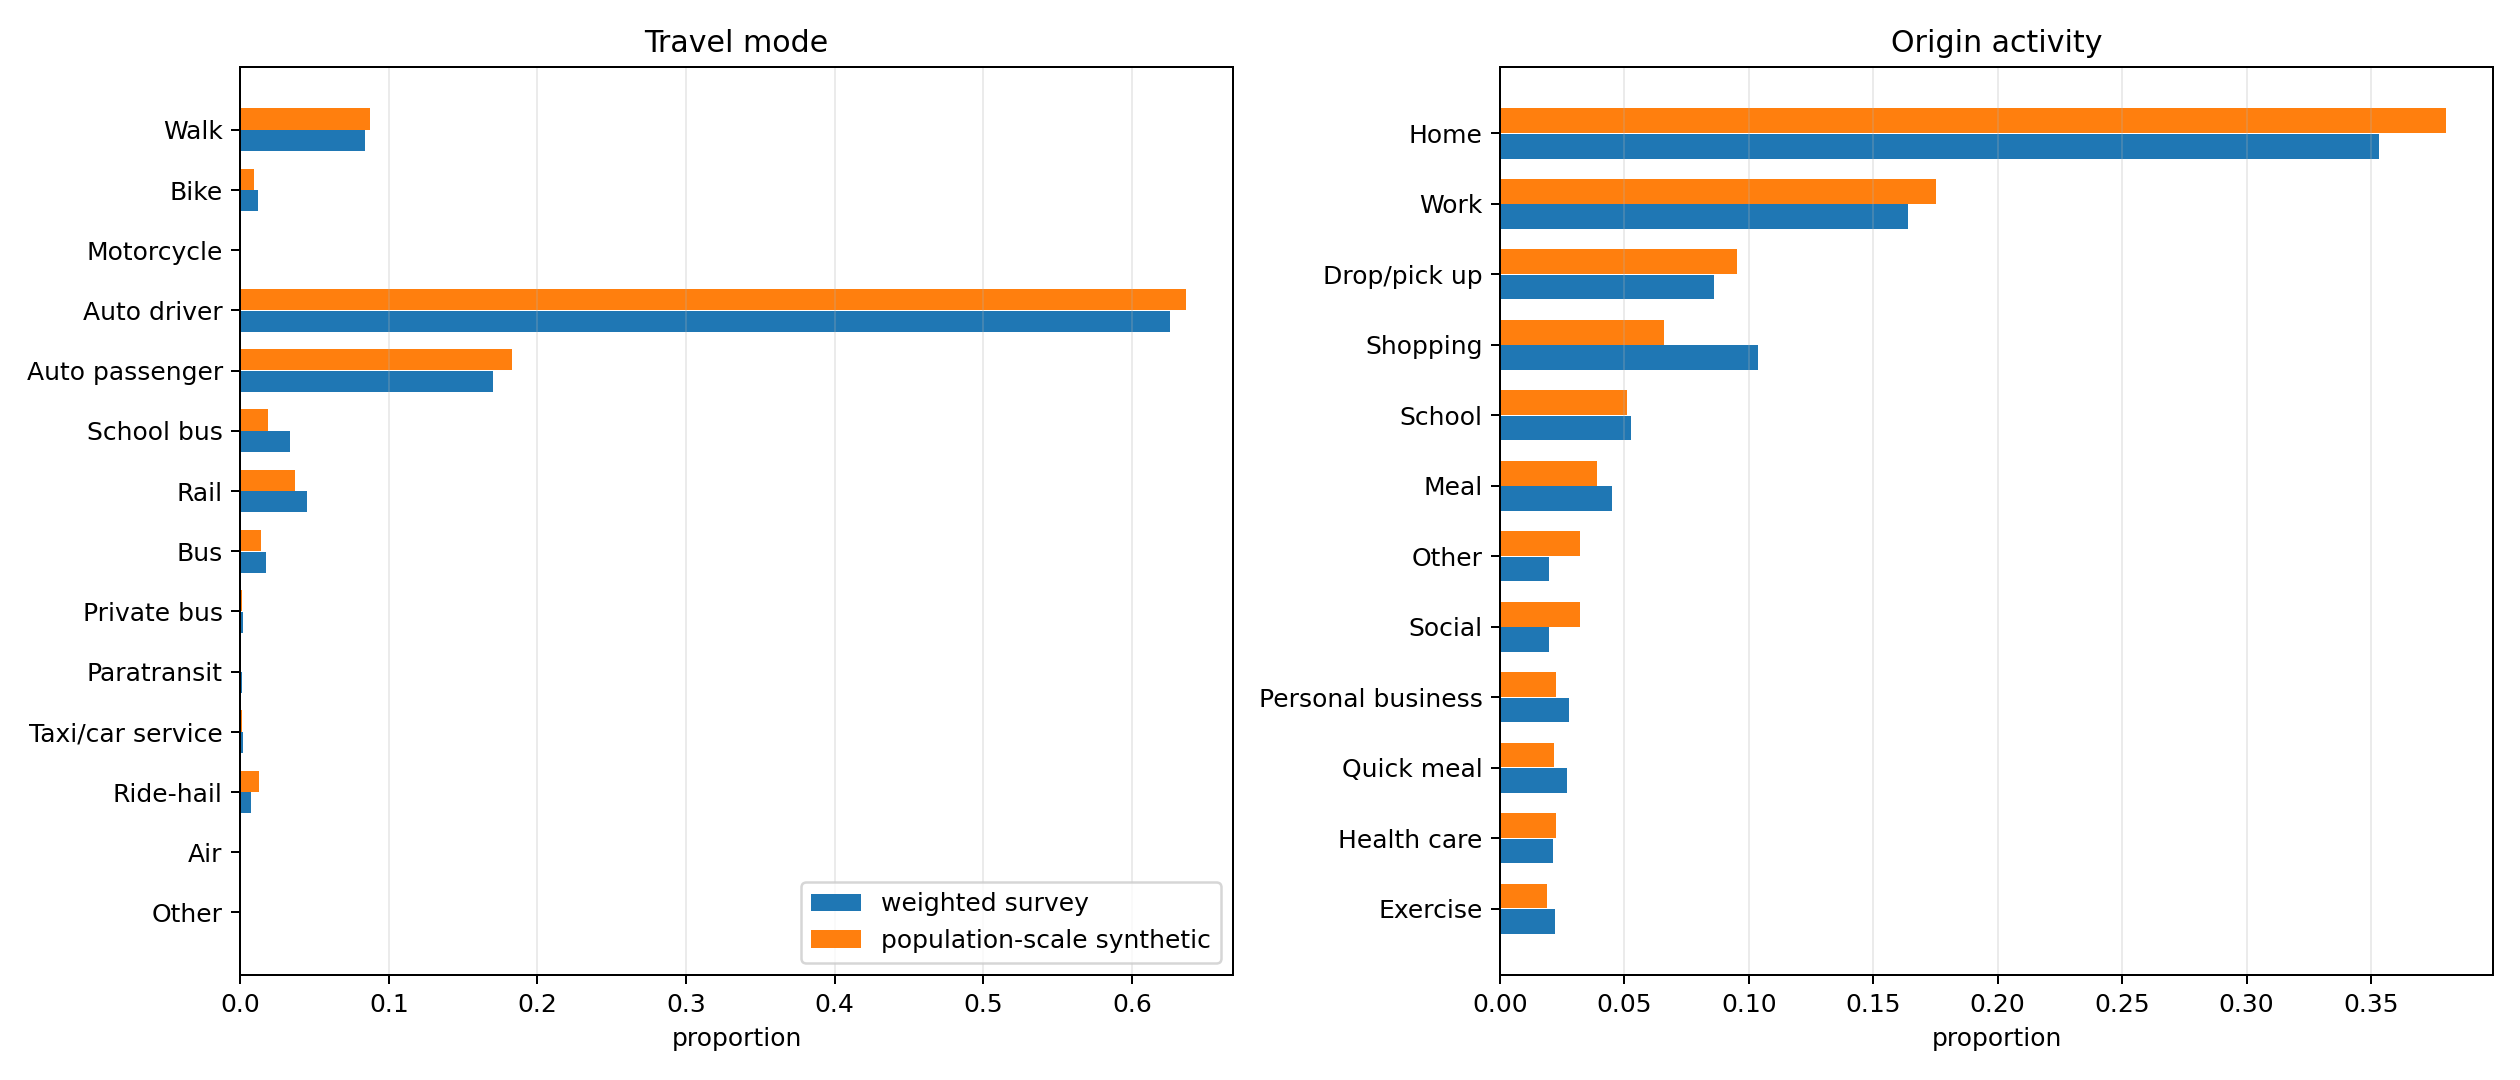
\includegraphics[width=.98\linewidth]{fig-labeled-mode-activity.png}
\caption{\textbf{Weighted survey and population-scale synthetic distributions for travel mode and origin activity.}}
\label{fig:labeled-mode-activity}
\end{figure}

Figure~\ref{fig:tvd-breakdown} ranks all modeled columns by total variation distance in the diagnostic synthetic sample. The most difficult variables are survey day, household size, and high-cardinality TAZ fields. Many binary, mode-access, vehicle, and demographic indicators have low total variation distance. This pattern indicates that the mixed-type VAE addresses the most severe categorical-encoding issue, but spatial sparsity remains a central modeling challenge.

\begin{figure}[H]
\centering
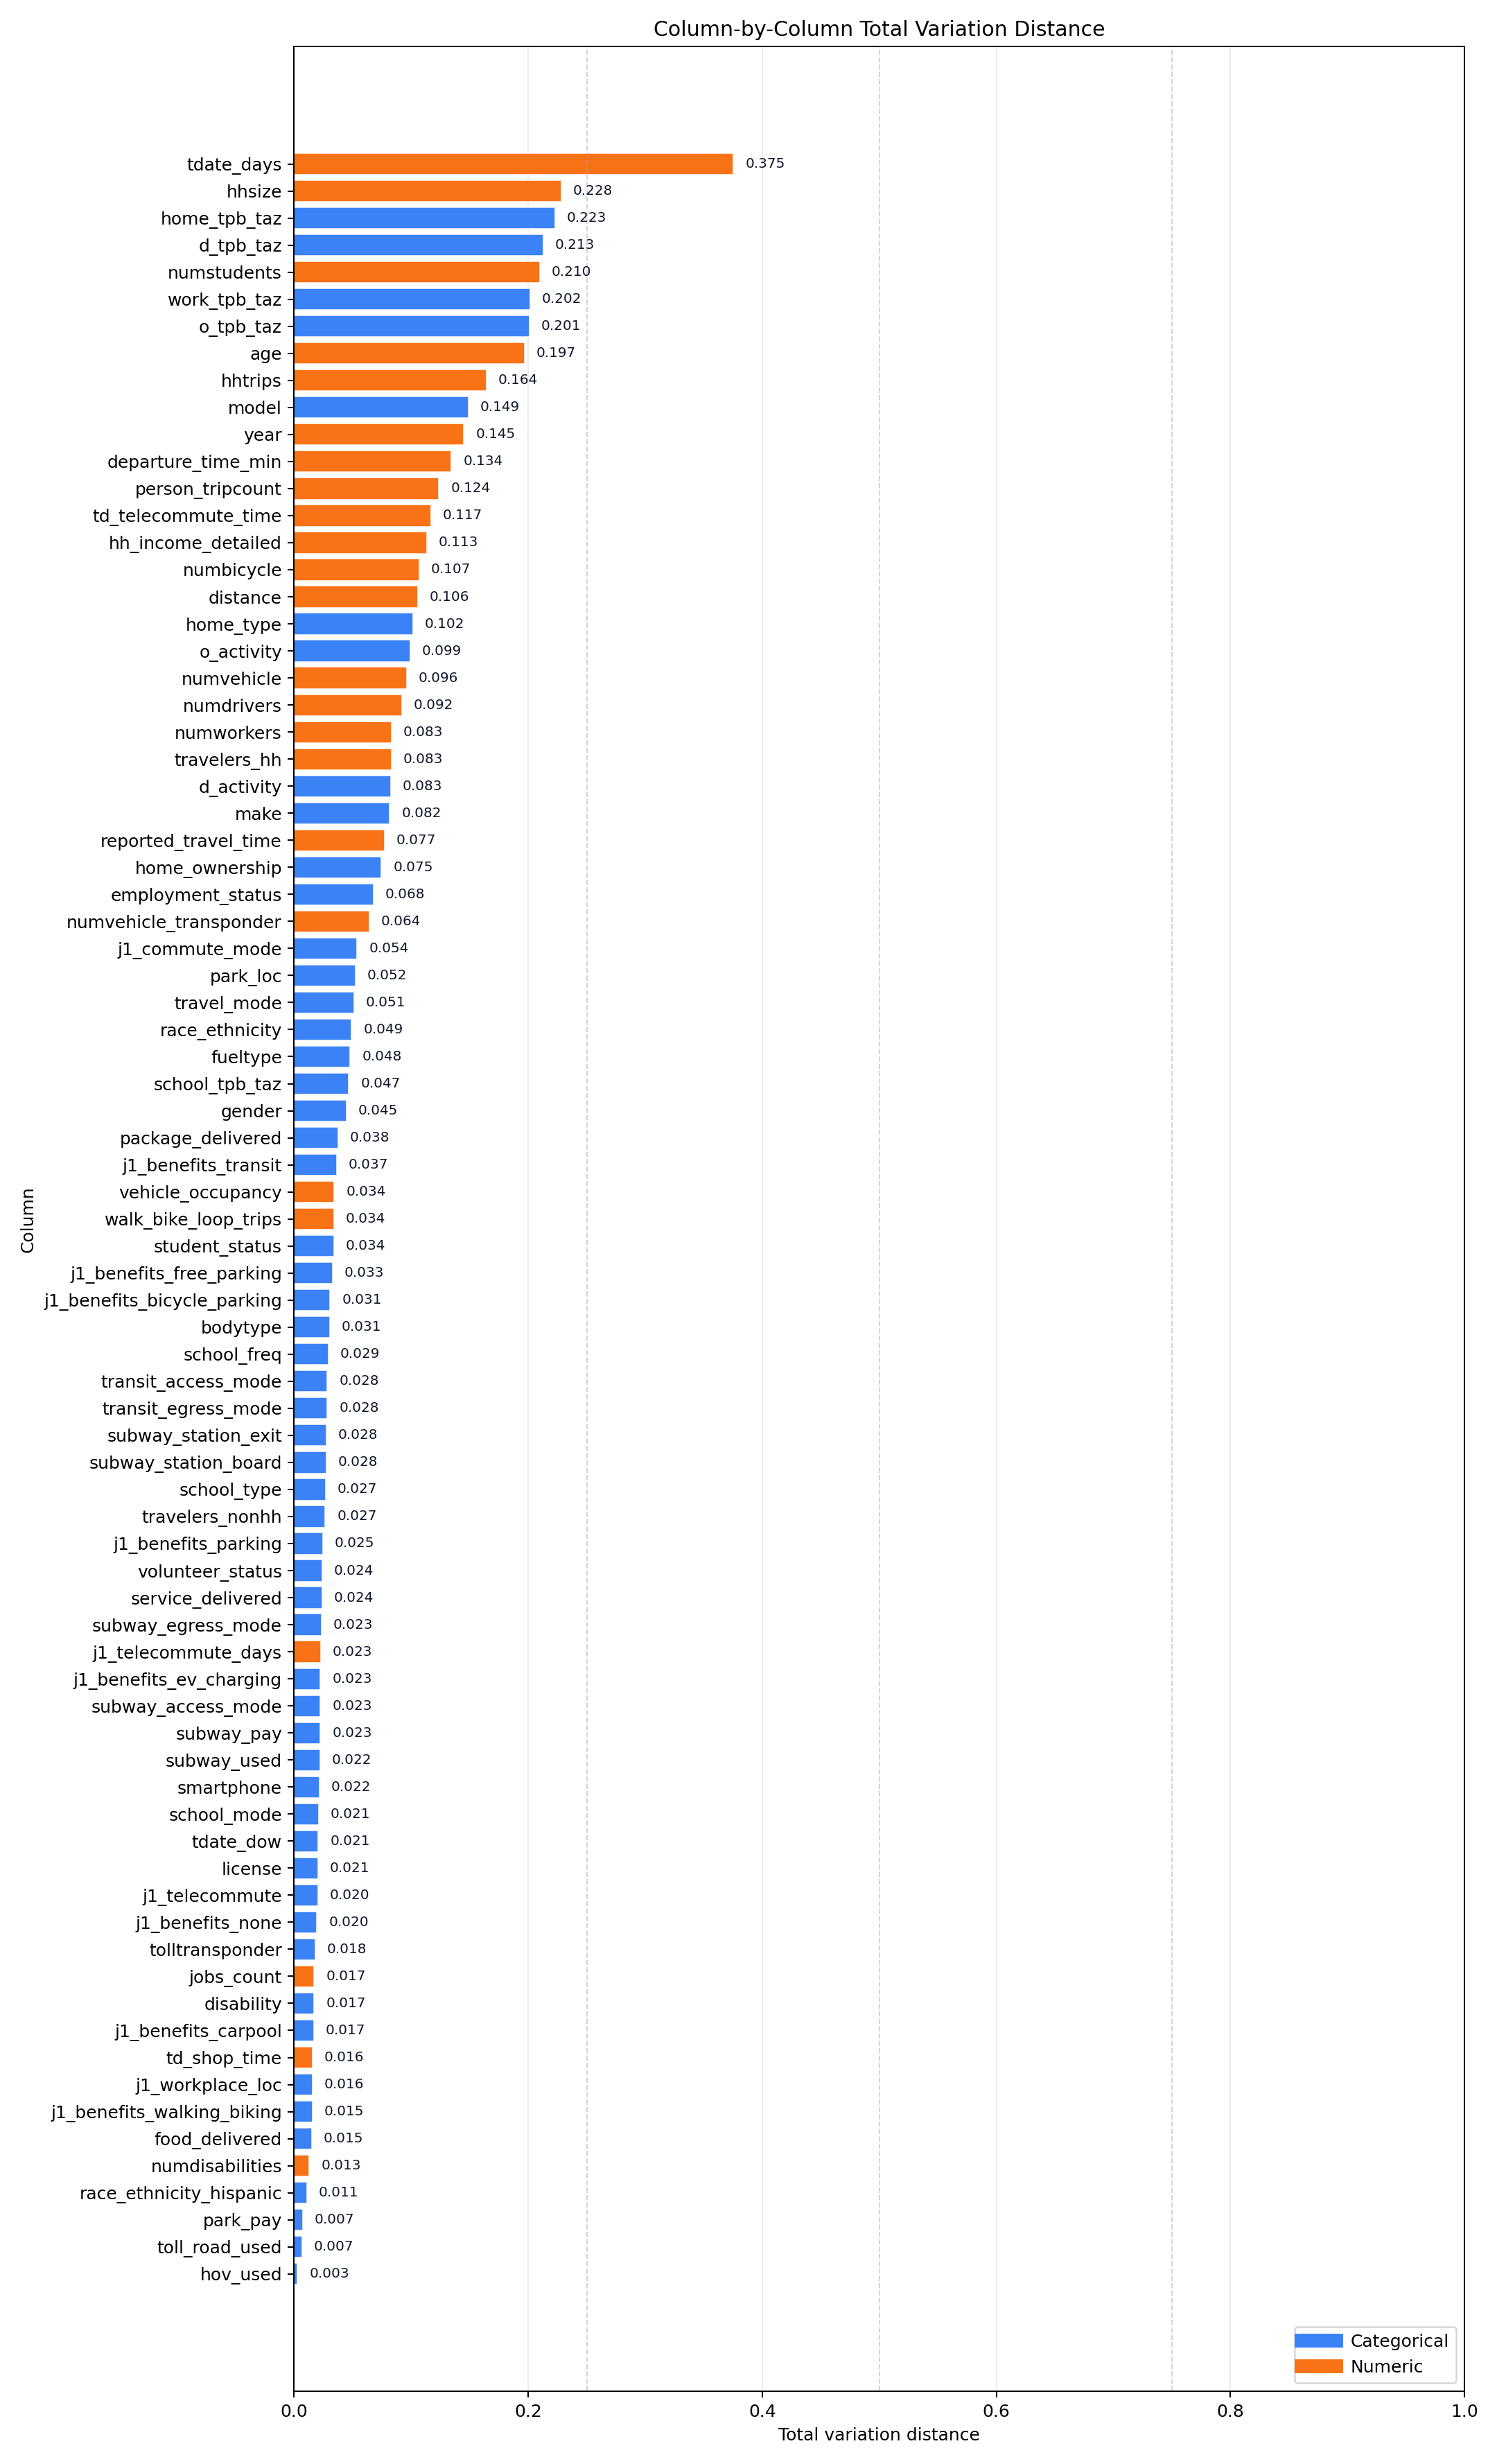
\includegraphics[width=.72\linewidth]{fig-total-variation-breakdown.png}
\caption{\textbf{Column-by-column total variation distance for the diagnostic synthetic sample.}}
\label{fig:tvd-breakdown}
\end{figure}

Pairwise cross-marginal validation shows the same limitation. Low-overlap pairs include TAZ-by-survey-day and origin--destination TAZ combinations, reflecting the high dimensionality and sparsity of the spatial fields. Consequently, the current model is best understood as a trip-microdata enrichment tool, not as a replacement for spatial control totals or calibrated origin--destination matrices.

\subsection{Revised MATSim Observed-Speed Validation}
The revised MATSim validation reports observed-speed errors as the primary road-assignment comparison. The pipeline writes three observed-speed products: the raw VDOT 511 segment snapshot, the OSM/MATSim link-matched observed speeds, and the real-versus-synthetic MATSim speed comparison. The key output files are \texttt{observed\_speeds\_raw.csv}, \texttt{observed\_speeds.csv}, \texttt{speed\_validation.csv}, and \texttt{speed\_validation\_summary.csv}.

The summary table produced by the rerun reports matched and modeled segment counts, observed mean speed, modeled mean speed, mean speed bias, MAE, RMSE, MAPE, Pearson correlation, and shares within 5~mph and 10~mph. The intended decision rule is direct: the VAE synthetic demand more clearly outperforms the weighted-survey sampling baseline only if it improves the main speed-error metrics and correlation under the same observed-speed match set. This focuses the external validation on directly observed operating speeds rather than proxy volume patterns.

The visualization bundle has also been revised for speed validation. It includes observed VDOT speed distributions, VDOT-to-OSM match-distance diagnostics, modeled-versus-observed speed scatter plots, and absolute speed-error histograms for the weighted-survey and VAE-synthetic scenarios. These figures should be regenerated after each feed pull because the public VDOT 511 data are time-varying operational observations.

\subsection{Scope and Limitations}
The revised methodology directly addresses several weaknesses of the earlier implementation. First, nominal variables are no longer treated as ordered integers under a global mean squared error loss. Second, population-scale trip counts are fixed by survey weights, avoiding the earlier issue of synthetic population totals drifting from known controls. Third, the VAE has a deeper encoder and decoder while using smaller training and sampling batches to reduce memory pressure. Fourth, the MATSim validation now uses directly observed travel speeds as the road-performance target.

Important limitations remain. The VAE is trained on the same broad survey geography used in validation, so the present experiments do not constitute a strict spatial hold-out transferability test. A stronger future design should train on selected geographies and evaluate on withheld areas with sufficient independent speed data. The public VDOT 511 feed is an operational snapshot, not a historical time-matched speed archive; future work should use NPMRDS, RITIS, probe-vehicle archives, or agency detector archives when licensed access is available. The current MATSim agents are single vehicle-trip agents located at TAZ centroids, not full-day household activity plans with within-zone location sampling. Mode choice is synthesized as an attribute but not modeled endogenously in MATSim. Finally, speed performance can still be weak without demand calibration, external origin--destination controls, and a complete regional multimodal network.

\section{Conclusion}
This paper presents a revised VAE-based trip synthesis pipeline that is better aligned with the statistical structure of household travel survey data. The key methodological change is mixed-type modeling: numeric variables are reconstructed continuously, while nominal categorical variables are embedded and trained with cross-entropy. Survey weights are used both during training and to set the population-scale sample size, so the VAE generates microstructure rather than population totals.

The population-scale synthetic dataset matches the weighted survey trip total by construction and reproduces many major univariate distributions, including travel mode, vehicle occupancy, activity purpose, and reported travel time. Spatial TAZ fields and sparse cross-marginals remain harder, which is expected in high-cardinality origin--destination synthesis. The revised MATSim validation is designed to test road-assignment realism against direct observed speeds, with the weighted survey expansion serving as the sampling baseline and the VAE synthetic demand as the competing input.

The results support a cautious interpretation: mixed-type VAEs are promising for enriching trip microdata, but they should be combined with known population controls, speed or volume calibration, external OD controls, and multimodal choice modeling before use in policy-sensitive forecasting. Future work should add explicit hold-out transferability tests, condition generation on external demographic and OD controls, sample coordinates within TAZ polygons, reconstruct full-day person plans, and include transit and mode-choice validation.

\section*{Acknowledgements}
ChatGPT was used during manuscript and code preparation to refine grammar, improve sentence structure, assist with code drafting, and generate preliminary summary text. All AI-assisted content was reviewed and edited by the authors, who take full responsibility for the final manuscript. The authors acknowledge support from the USDOT Center for Multimodal Mobility in Urban, Rural, and Tribal Areas (CMMM) at the University of Maryland.

\section*{Author Contributions}
Study conception and design: Cinzia Cirillo, Darshan Pandit, Raziq Zaman. Data collection and preparation: Raziq Zaman, Raas Sarker Tomal, Md Mahmudul Huque Chayan. Analysis and interpretation of results: Md Mahmudul Huque Chayan, Raziq Zaman, Raas Sarker Tomal. Draft manuscript preparation: Raziq Zaman, Md Mahmudul Huque Chayan, Raas Sarker Tomal, Darshan Pandit. All authors reviewed the results and approved the final version of the manuscript.

\section*{Declaration of Conflicting Interests}
The authors declared no potential conflicts of interest with respect to the research, authorship, and/or publication of this article.

\bibliographystyle{elsarticle-num}
\bibliography{references}

\end{document}
